\documentclass{article}

% Language and encoding settings
\usepackage[utf8]{inputenc}
\usepackage[T1]{fontenc}

% Essential packages
\usepackage{graphicx}      % For importing images
\usepackage{amsmath,amssymb} % For mathematical formatting
\usepackage{booktabs}      % For professional tables
\usepackage{hyperref}      % For clickable links and cross-reference
\usepackage{subcaption}

% Metadata
\title{Micro-VLA: Scaling In-Context Robotic Manipulation via Observation-Only Videos \footnote{We dropped the "via Observation-Only Videos", as discussed with our lab teacher.}}
\author{Adrian Boguszewski, Bartosz Czechowski}
\date{\today}

\begin{document}

\maketitle

\section*{Opening Remarks}
Throughout the report, the model that we are discussing is not a VLA.
Initially we experimented with a pretrained, 500M parameter VLA - \href{https://huggingface.co/lerobot/smolvla\_base}{\textit{SmolVLA}}, however we quickly realized that it wasn't computationally feasible for us.
One epoch of fine-tuning the action head (not even the VLM backbone) took around an hour on a Google Colab T4 GPU, and yielded around 10\% success rate on the simplest task we were interested in.
We decided to train an order of magnitude smaller decision transformer from scratch (whose architecture will be disclosed in a later section).

\section{The Environments}
We decided to use \href{https://robosuite.ai/}{\textit{robosuite}}, which its authors describe as "a simulation framework powered by the MuJoCo physics engine for robot learning (...) (that) also offers a suite of benchmark environments for reproducible research".
The decision was motivated by its easily configurable environments with an option to swap out robot arms to any of the available models.

\subsection{Tasks}
We chose a subset of three tasks, based on the following criteria: they have an obvious difficulty ordering, they can be seen as a natural extension of one another, and they have accompanying dataset (with an asterisk described in a later section).

\subsubsection{Block Lifting}
A cube is placed on the tabletop in front of a single robot arm.
The robot arm must lift the cube above a certain height.
The cube's location is randomized at the beginning of each episode.
\begin{figure}[htbp]
  \centering
  \begin{subfigure}[b]{0.20\textwidth}
    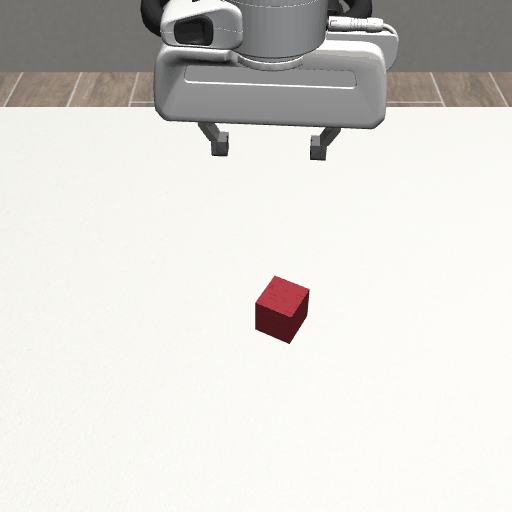
\includegraphics[width=\textwidth]{images/lift/demo-11.png}
  \end{subfigure}%
  \begin{subfigure}[b]{0.20\textwidth}
    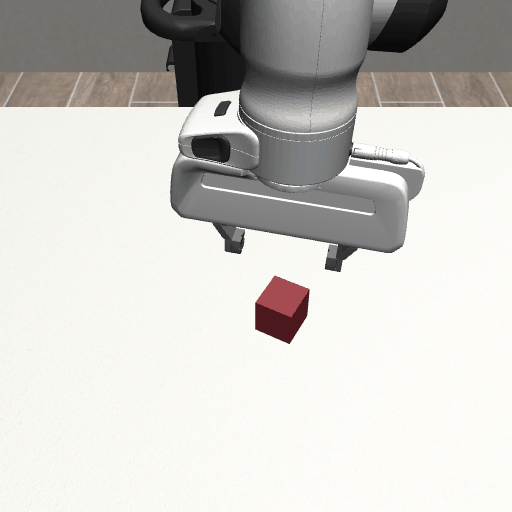
\includegraphics[width=\textwidth]{images/lift/demo-22.png}
  \end{subfigure}%
  \begin{subfigure}[b]{0.20\textwidth}
    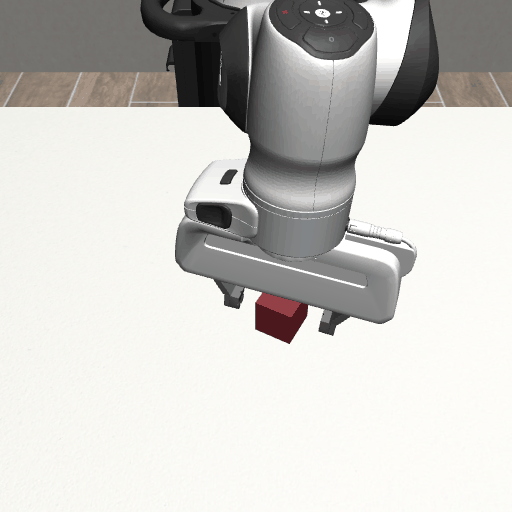
\includegraphics[width=\textwidth]{images/lift/demo-33.png}
  \end{subfigure}%
  \begin{subfigure}[b]{0.20\textwidth}
    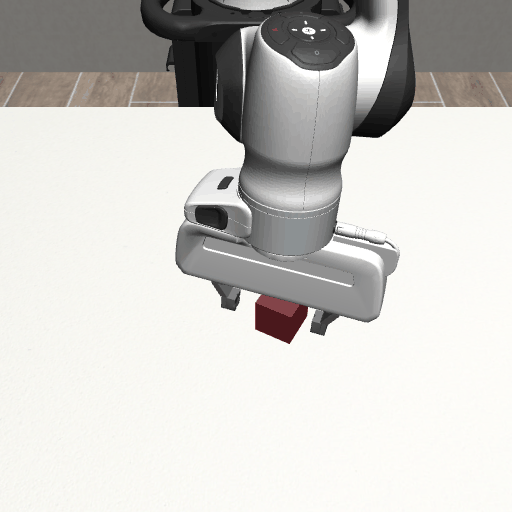
\includegraphics[width=\textwidth]{images/lift/demo-44.png}
  \end{subfigure}%
  \begin{subfigure}[b]{0.20\textwidth}
    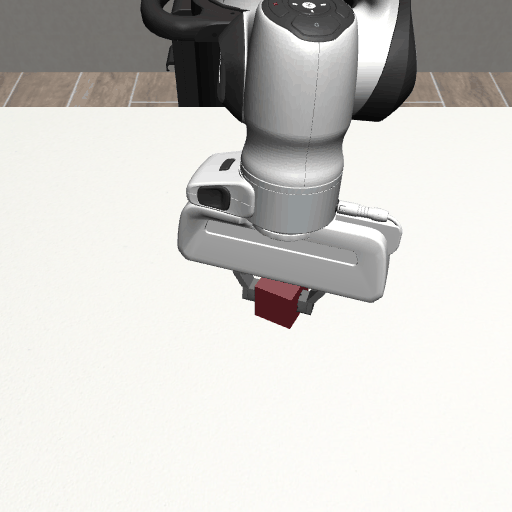
\includegraphics[width=\textwidth]{images/lift/demo-55.png}
  \end{subfigure}%
  \caption {\textit{Block Lifting} task demonstration}
\end{figure}

\subsubsection{Block Stacking}
Two cubes (red and green) are placed on the tabletop in front of a single robot arm.
The robot must place the red cube on top of the green cube.
The cubes' locations are randomized at the beginning of each episode.
\begin{figure}[htbp]
  \centering
  \begin{subfigure}[b]{0.20\textwidth}
    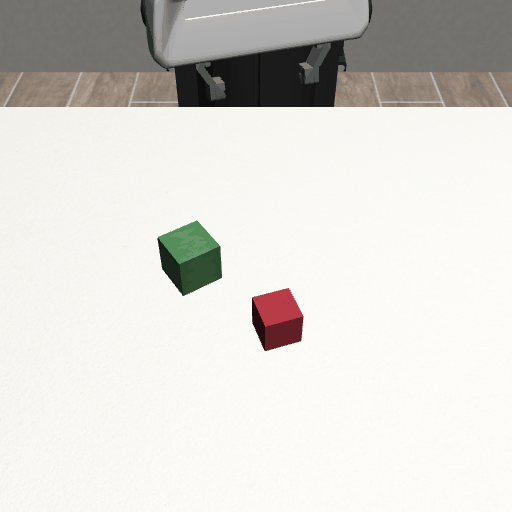
\includegraphics[width=\textwidth]{images/stack/demo-19.png}
  \end{subfigure}%
  \begin{subfigure}[b]{0.20\textwidth}
    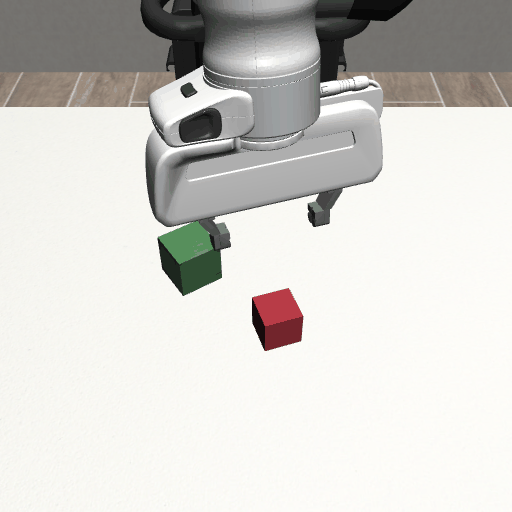
\includegraphics[width=\textwidth]{images/stack/demo-38.png}
  \end{subfigure}%
  \begin{subfigure}[b]{0.20\textwidth}
    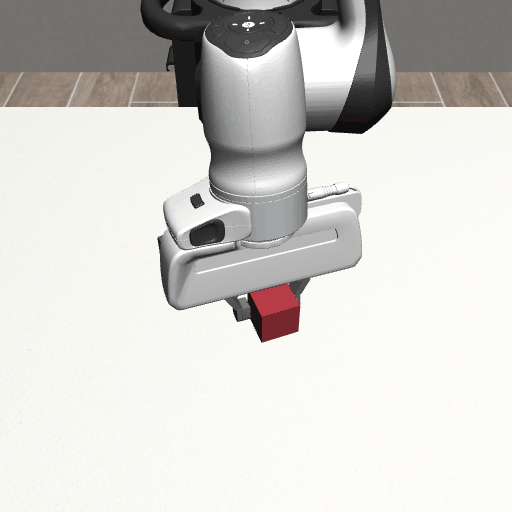
\includegraphics[width=\textwidth]{images/stack/demo-57.png}
  \end{subfigure}%
  \begin{subfigure}[b]{0.20\textwidth}
    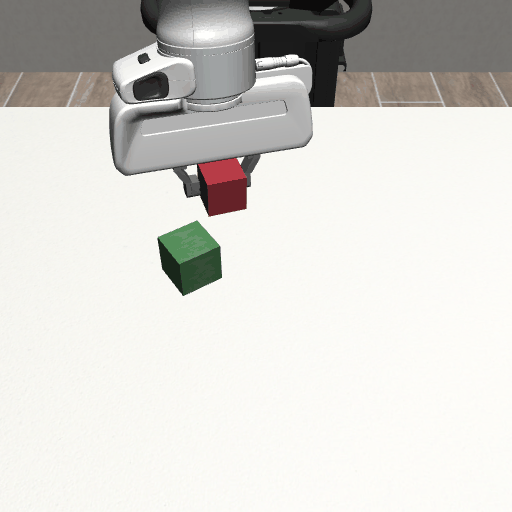
\includegraphics[width=\textwidth]{images/stack/demo-76.png}
  \end{subfigure}%
  \begin{subfigure}[b]{0.20\textwidth}
    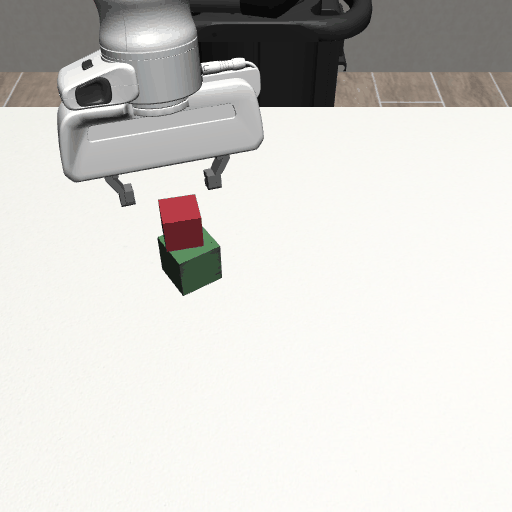
\includegraphics[width=\textwidth]{images/stack/demo-95.png}
  \end{subfigure}%
  \caption {\textit{Block Stacking} task demonstration}
\end{figure}

\subsubsection{Nut Assembly (one square nut variant)}
Two colored pegs (one square and one round) are mounted on the tabletop, and a square nut is placed on the table in front of a single robot arm.
The robot must fit the square nut onto the square peg.
The nut's location is randomized at the beginning of each episode, while the pegs are fixed.
\begin{figure}[htbp]
  \centering
  \begin{subfigure}[b]{0.20\textwidth}
    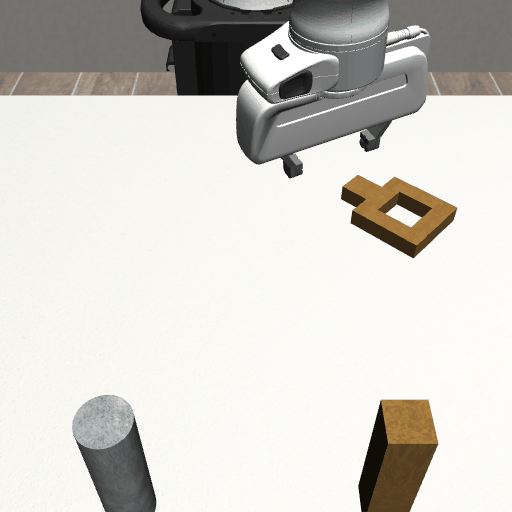
\includegraphics[width=\textwidth]{images/nut/demo-25.png}
  \end{subfigure}%
  \begin{subfigure}[b]{0.20\textwidth}
    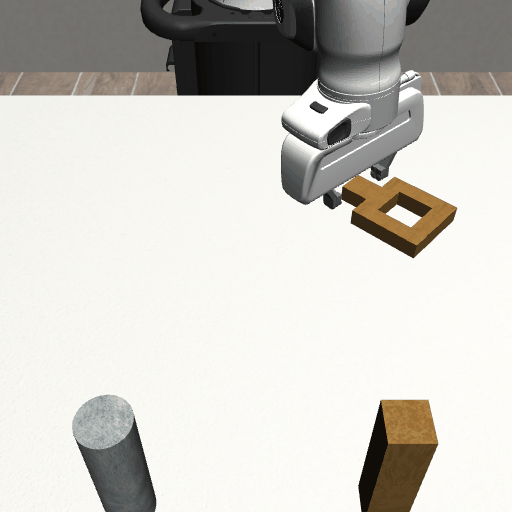
\includegraphics[width=\textwidth]{images/nut/demo-50.png}
  \end{subfigure}%
  \begin{subfigure}[b]{0.20\textwidth}
    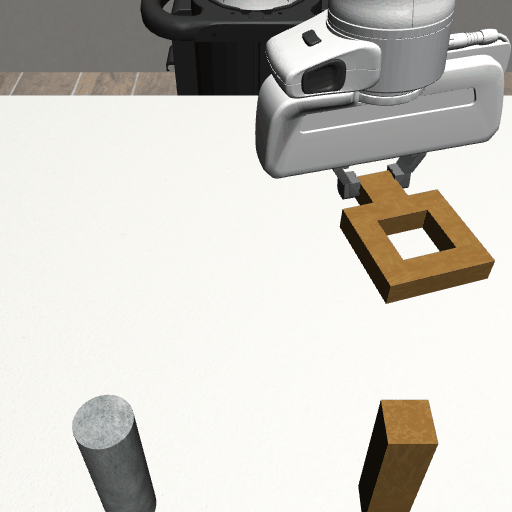
\includegraphics[width=\textwidth]{images/nut/demo-75.png}
  \end{subfigure}%
  \begin{subfigure}[b]{0.20\textwidth}
    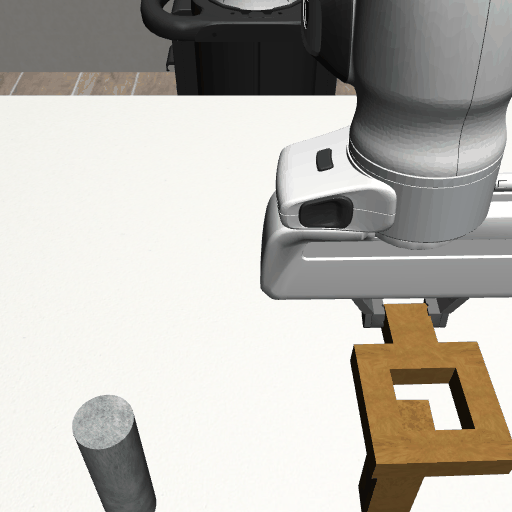
\includegraphics[width=\textwidth]{images/nut/demo-100.png}
  \end{subfigure}%
  \begin{subfigure}[b]{0.20\textwidth}
    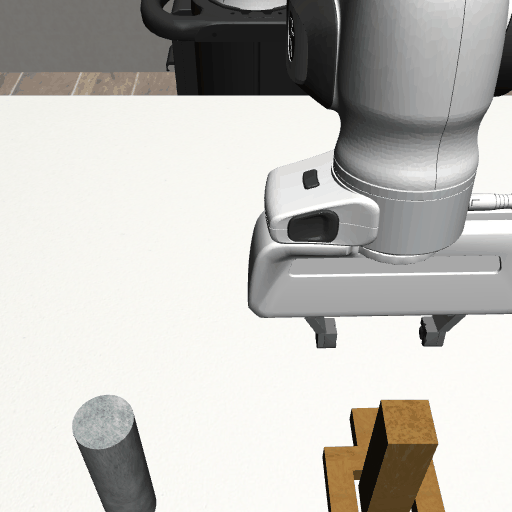
\includegraphics[width=\textwidth]{images/nut/demo-125.png}
  \end{subfigure}%
  \caption {\textit{Nut Assembly} task demonstration}
\end{figure}


\subsection{Robot Arms}
Throughout the project we use two robot arms: Panda and IIWA.
The first one was chosen, because it was present in the datasets that we had access to (described later).
The second one was selected for its similarity to the Panda - 6 degrees of freedom with similar kinematics and a single-degree-of-freedom gripper.
Two distinct arms were necessary to evaluate cross-embodiment generalization.

\begin{figure}[htbp]
  \centering
  \begin{minipage}[b]{0.48\textwidth}
    \centering
    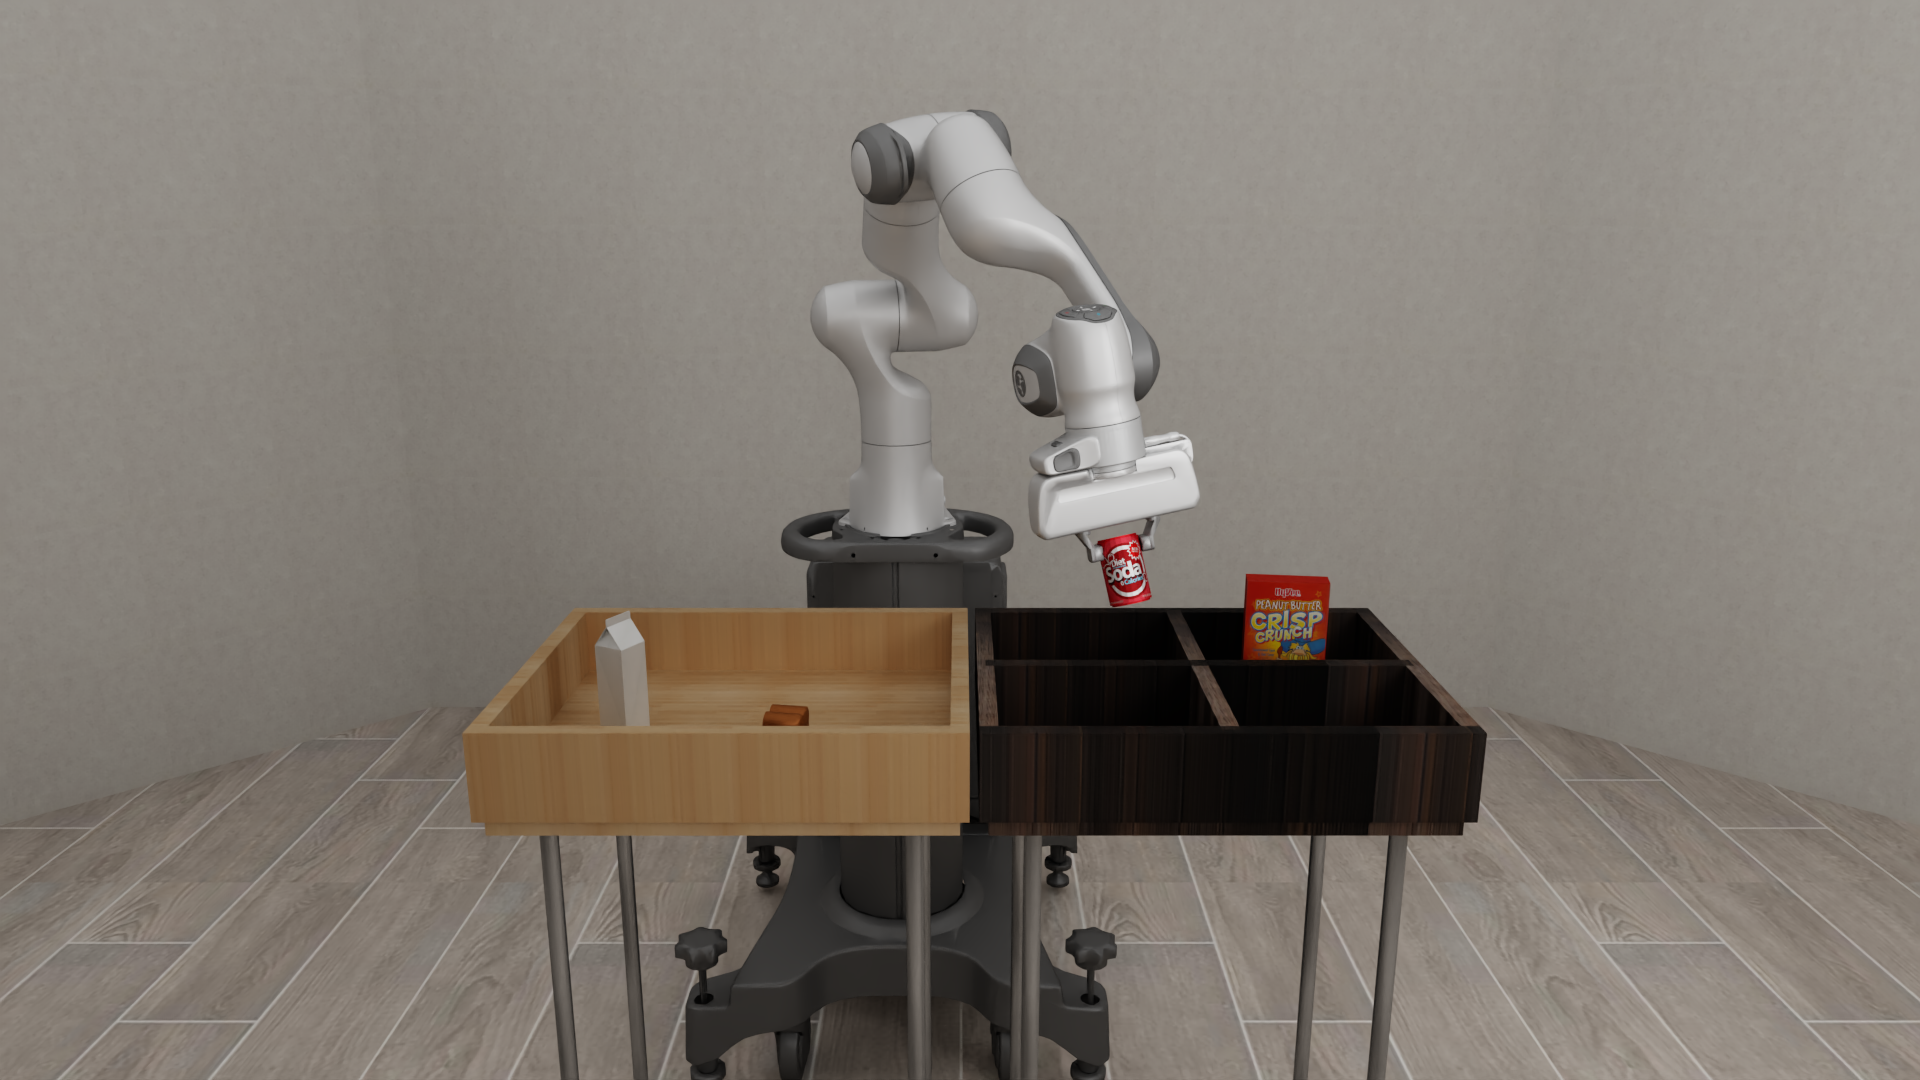
\includegraphics[width=\textwidth]{images/arms/panda.png}
    \caption{Panda arm}
  \end{minipage}
  \hfill
  \begin{minipage}[b]{0.48\textwidth}
    \centering
    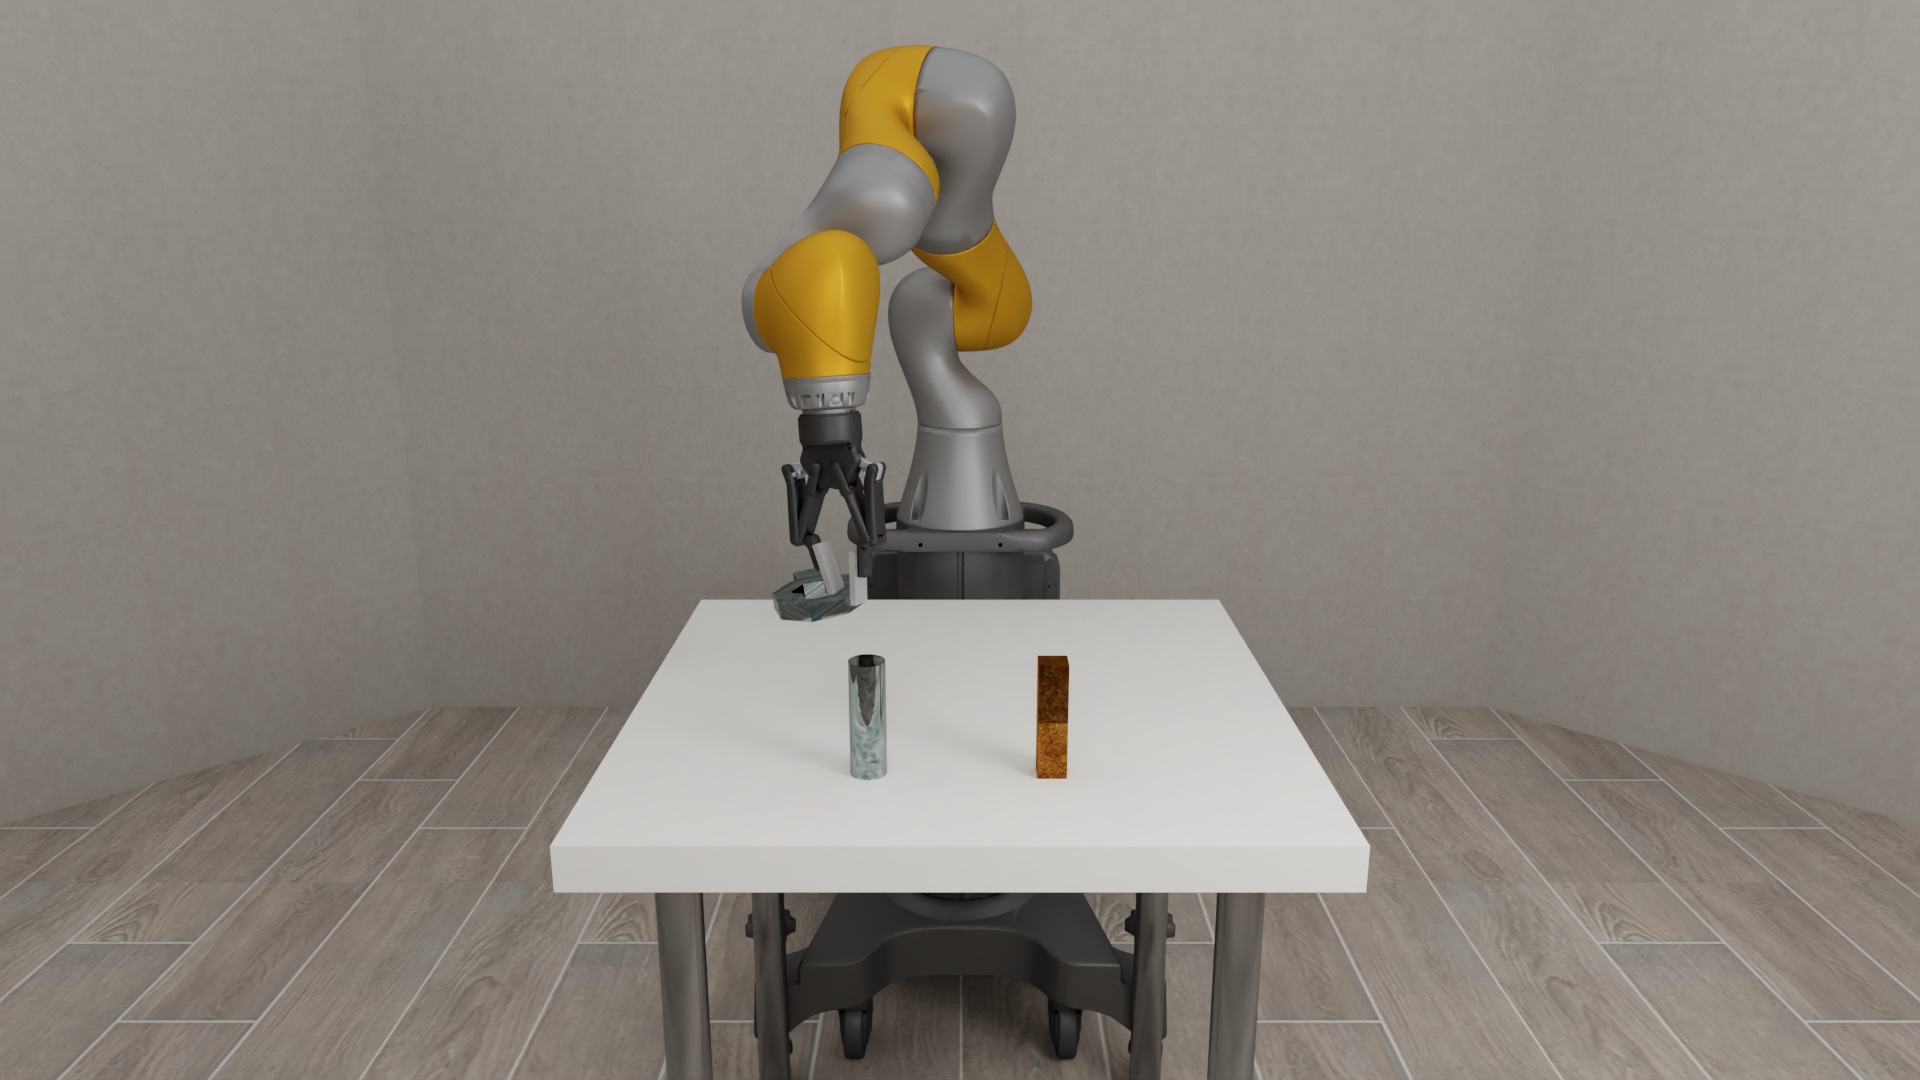
\includegraphics[width=\textwidth]{images/arms/iiwa.png}
    \caption{IIWA arm}
  \end{minipage}
\end{figure}

\section{Training Data}
As our training data we mainly used demonstrations sourced from \href{https://huggingface.co/datasets/robomimic/robomimic_datasets}{\textit{robomimic}}.
In its totality, \textit{robomimic} is a more general framework, but we used it solely as a source of human demonstrations and dataset processing scripts.

From \textit{robomimic} we took proficient human and multi-human (divided into "better", "okay" and "worse" operators) demonstrations for block lifting and nut assembly tasks (using the Panda arm),
as well as the machine generated trajectories for block lifting (again, using the Panda arm).

What we couldn't find in \textit{robomimic's} archive, we collected ourselves - block stacking demonstrations (using Panda and IIWA arms), and block lifting demonstrations for the IIWA arm.

We also had to process those datasets to prepare the camera observations, rewards, and feature extractor embeddings of the camera observations for training efficiency (the feature extractor is described in the following section).
The original datasets only contained raw trajectories (action, joint and environment state sequences).

All of our training data is publicly available on \href{https://huggingface.co/datasets/aboguszewski/robomimic}{\textit{HuggingFace}} with a comprehensive dataset card that goes into more technical details.

\section{Model Architecture}
We used  a rather standard Decision Transformer architecture - with some implementation details described below.
The whole implementation of this project is available on \href{https://github.com/czechuuu/micro-vla}{GitHub}.
\subsection{Rewards}
We made using rewards optional - as when learning from expert trajectories they don't carry much information.
But if one decides to use rewards (possibly due to introducing sub-optimal trajectories in the dataset), it's configurable whether to use the dense rewards from the dataset (which grow as the model gets closer to the goal) or to use time based rewards (where we give a reward of -1 at every step, and +100 on success).
Then these rewards are used in the return-to-go fashion from the original Decision Transformer paper.

Using dense rewards is sub-optimal as it can be misleading - a model that takes longer to pick up the cube will get a higher total episode return than a model that picks it up faster.

\subsection{Observations}
As input the model takes a proprioception vector (end-effector position, end-effector rotation, gripper width) and two precomputed Dino3 ViT-Small embeddings of the images from two cameras (eye in hand and robotview).
It can be configured whether these should be concatenated into one vector which will be embedded into the latent space of the model, or whether they should be embedded separately and then attended to separately by the model.

We have found that fusing the observations into one gives better results than attending to them separately.

\subsection{In-context learning}
We also implemented in-context learning - where we also provide the model with a successful trajectory of the task (during training and evaluation).

\subsection{Positional Embeddings}
We have decided to use learnable positional embeddings as in the original Decision Transformer paper. 
When using in-context learning we have decided to reset the timestep counter to zero.

Using sinusoidal positional embeddings and not resetting the timestep counters were considered but not evaluated.

\subsection{Training}
We have implemented a standard training loop with MSE loss. We have enabled training on multiple datasets with configurable weighed sampling. 

\subsection{Initial Experiment}
We performed an initial experiment to test whether this architecture was capable of learning the simplest of our tasks - block lifting.
The experiment was successful (see Figure 6), however we came across a weird phenomenon (also described in the original \textit{robomimic} paper).
The validation loss didn't correlate with model's performance inside the environment.
This meant that for every experiment we had to perform validation rollouts inside the environment to accurately grasp model progress,
and that it is worth to train the model much longer than we initially thought.

Another important thing to note is that the training is really unstable and the evaluation carries great variance.

\begin{figure}[htbp]
    \centering
    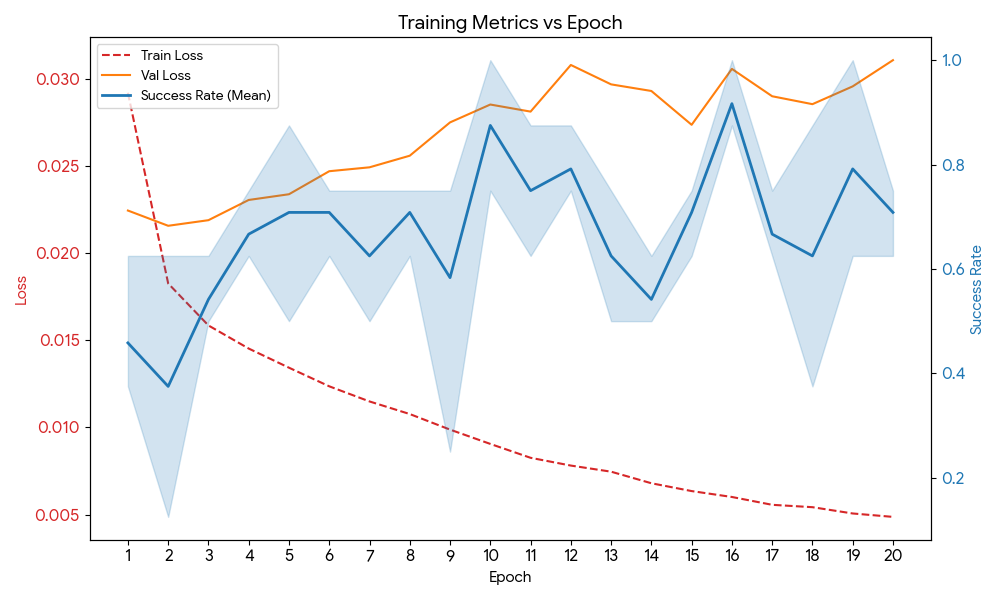
\includegraphics[width=\textwidth]{images/plots/non_icl_variance_graph.png}
    \caption{Training and validation losses, as well as success rates plotted against the training epochs on the block lifting task.}
\end{figure}

\section{Task Generalization}
We performed a large number of experiments that tested generalization between tasks.

\subsection{Color Change}
A model trained on the block lifting task with a red cube exhibited equal zero-shot performance on cubes of different colors (see Figure 7).
However, after inspecting the actual produced trajectories (also failures) we noticed that unfortunately it's not true generalization,
but instead overfitting to block position (a recurring problem in this project).

\begin{figure}[htbp]
    \centering
    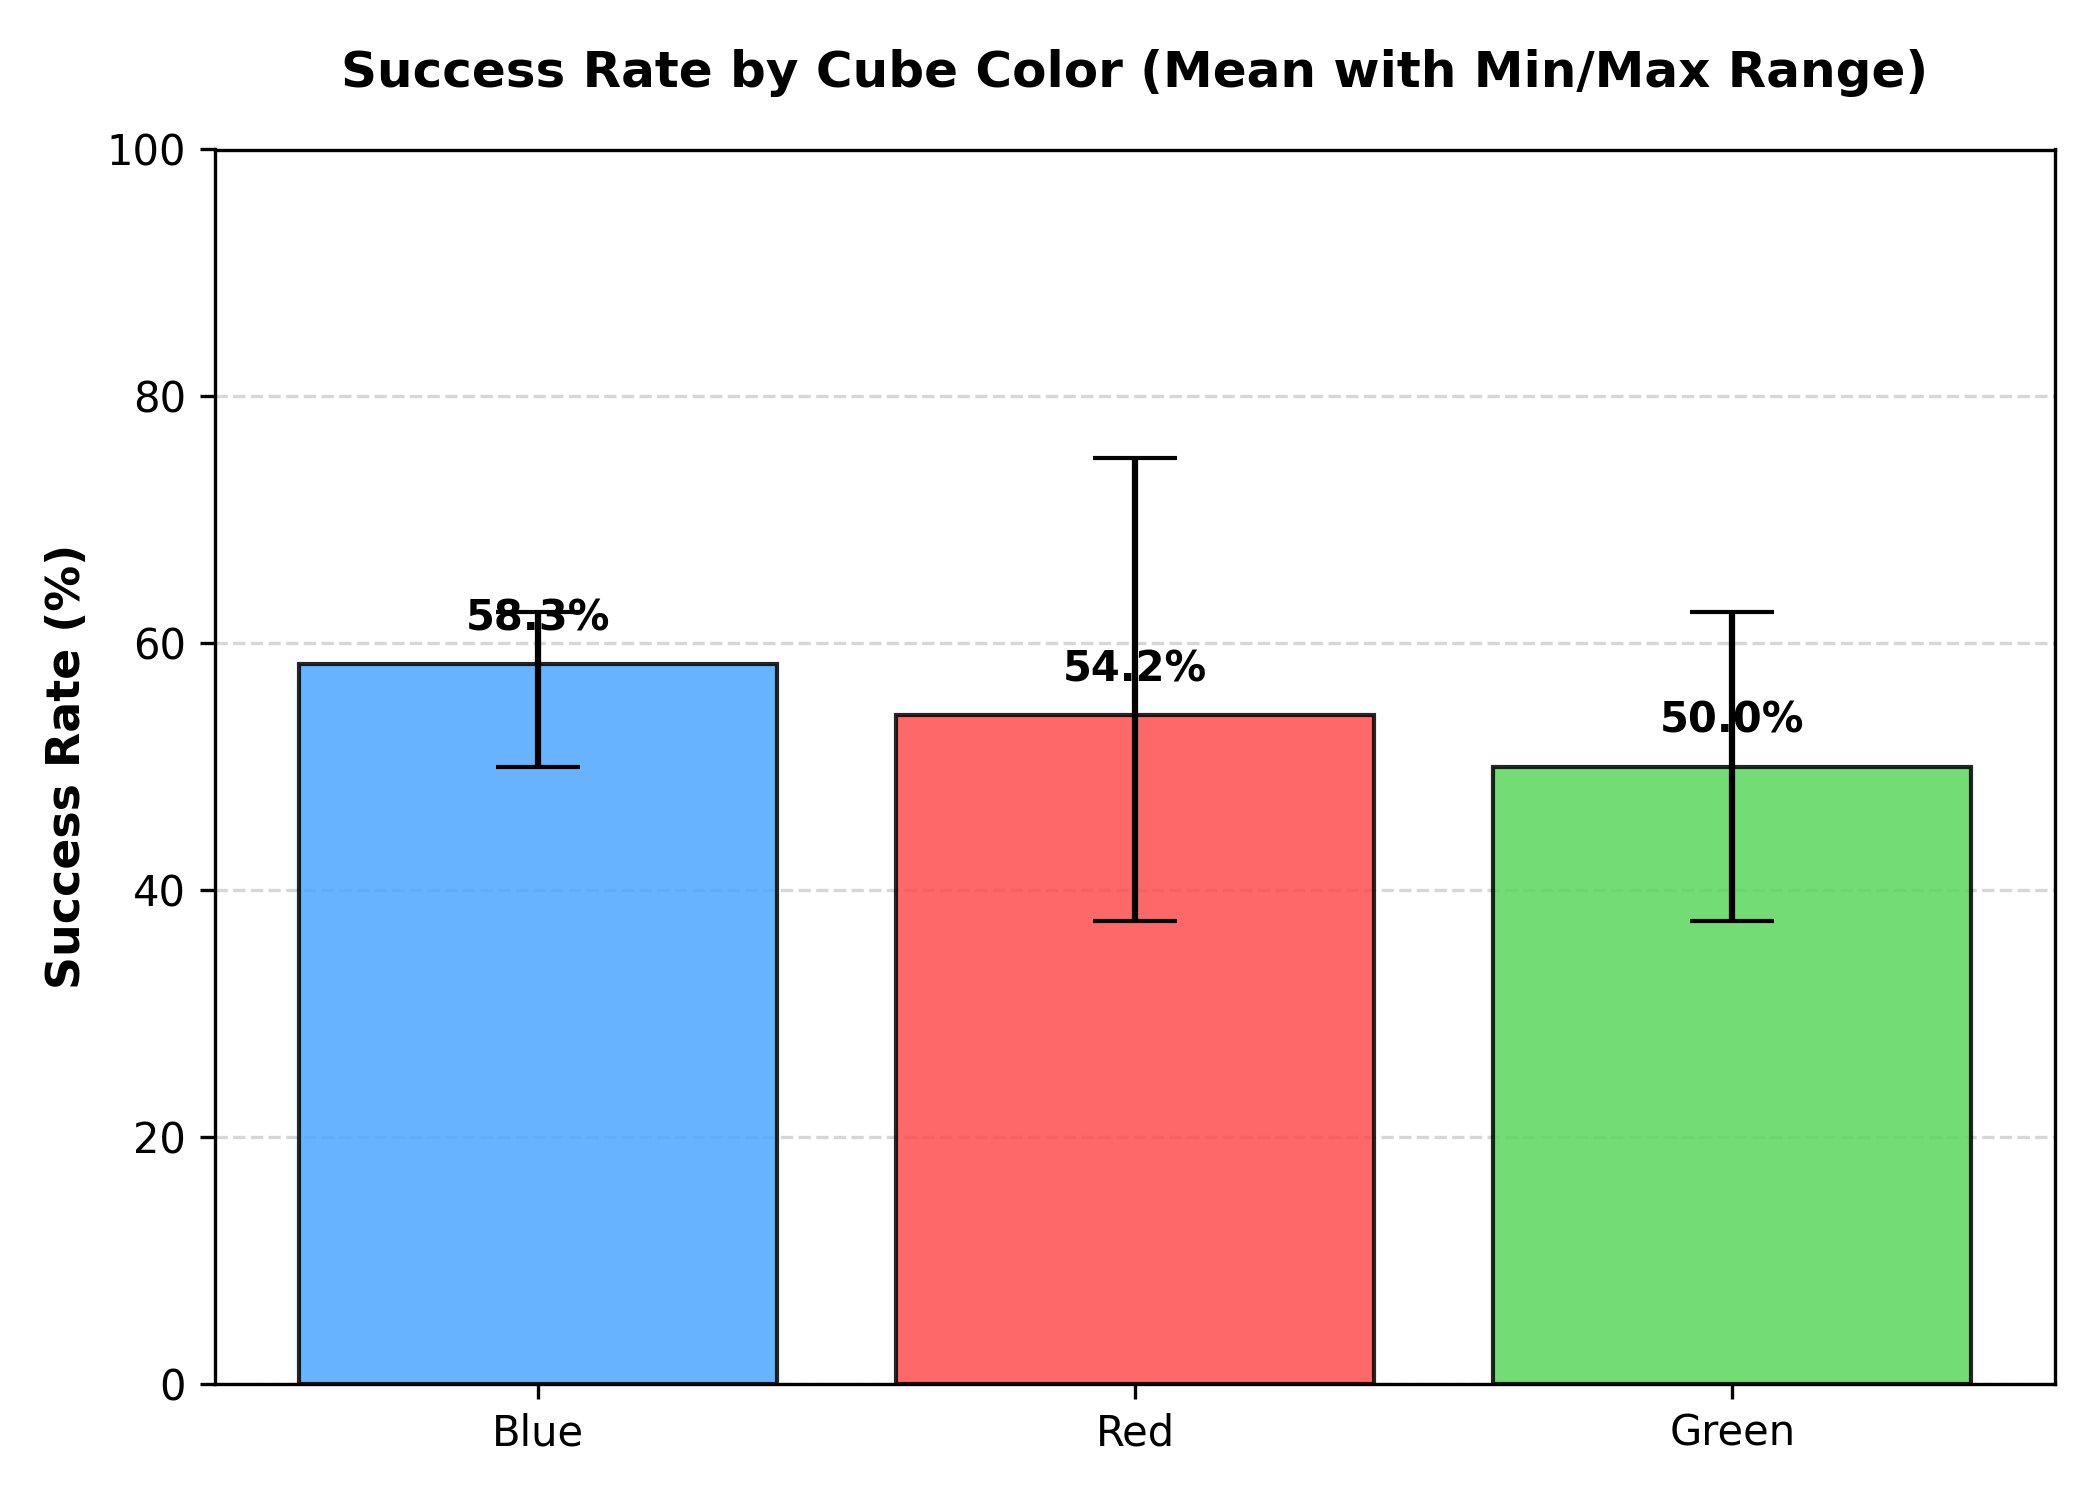
\includegraphics[width=\textwidth]{images/plots/multi_colour.png}
    \caption{Model performance on different cube colors.}
\end{figure}

\subsection{Training with In-Context Prompts}
A model trained with in-context prompts didn't achieve better one-shot performance than a baseline zero-shot model on the trained task
(see Figure 8 and remember that the best version of the initial model scored $\sim$ 90\%).

\begin{figure}[htbp]
    \centering
    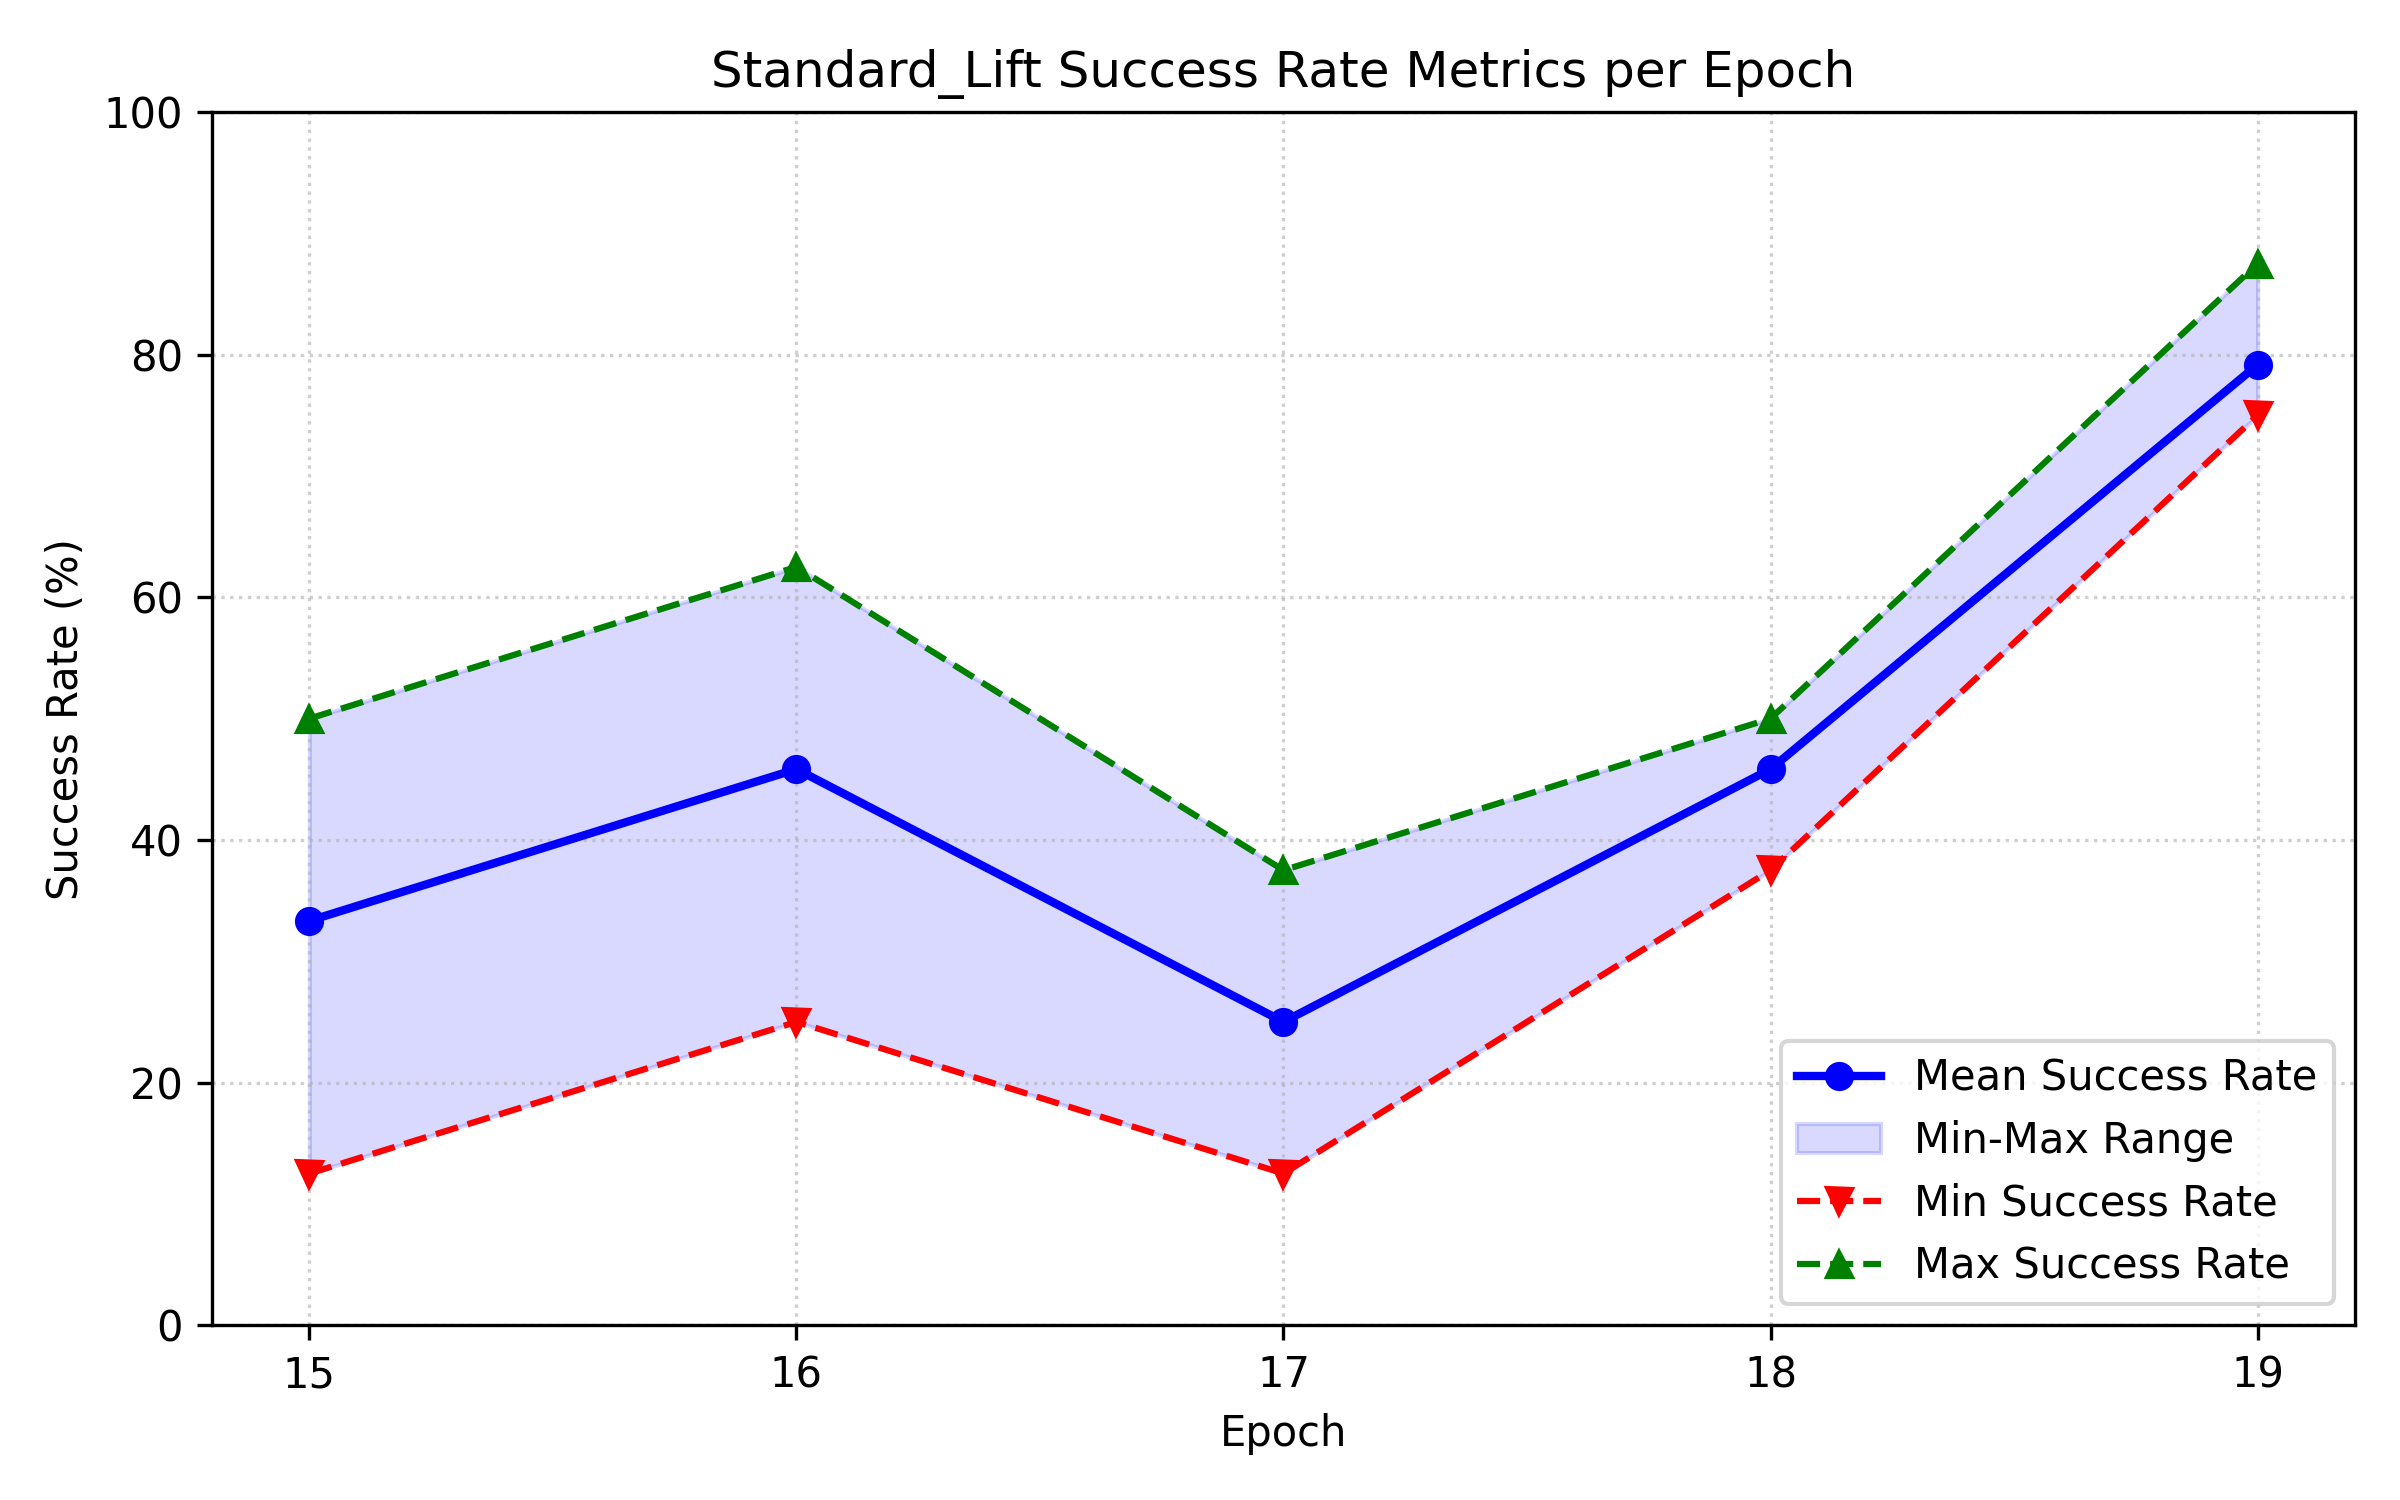
\includegraphics[width=\textwidth]{images/plots/baseline_icl.png}
    \caption{Performance of the model trained with in-context prompts on the block lifting task.}
\end{figure}

\subsection{Scaling Up Training with In-Context Prompts}
Introducing time-based rewards (-1 for each step and +100 for success) and increasing the size of training data degraded performance on the trained task.
The dataset was extended with demonstrations of lower quality - multi-human (MH), so datasets collected by multiple human operators of varying proficiency level, and machine generated ones (MG).
Previously the models were trained on proficient human (PH) demonstrations.
For the exact results see Figures 9, 10, 11.
Adding demonstrations of the nut assembly task also failed to produce any results.

\begin{figure}[htbp]
    \centering
    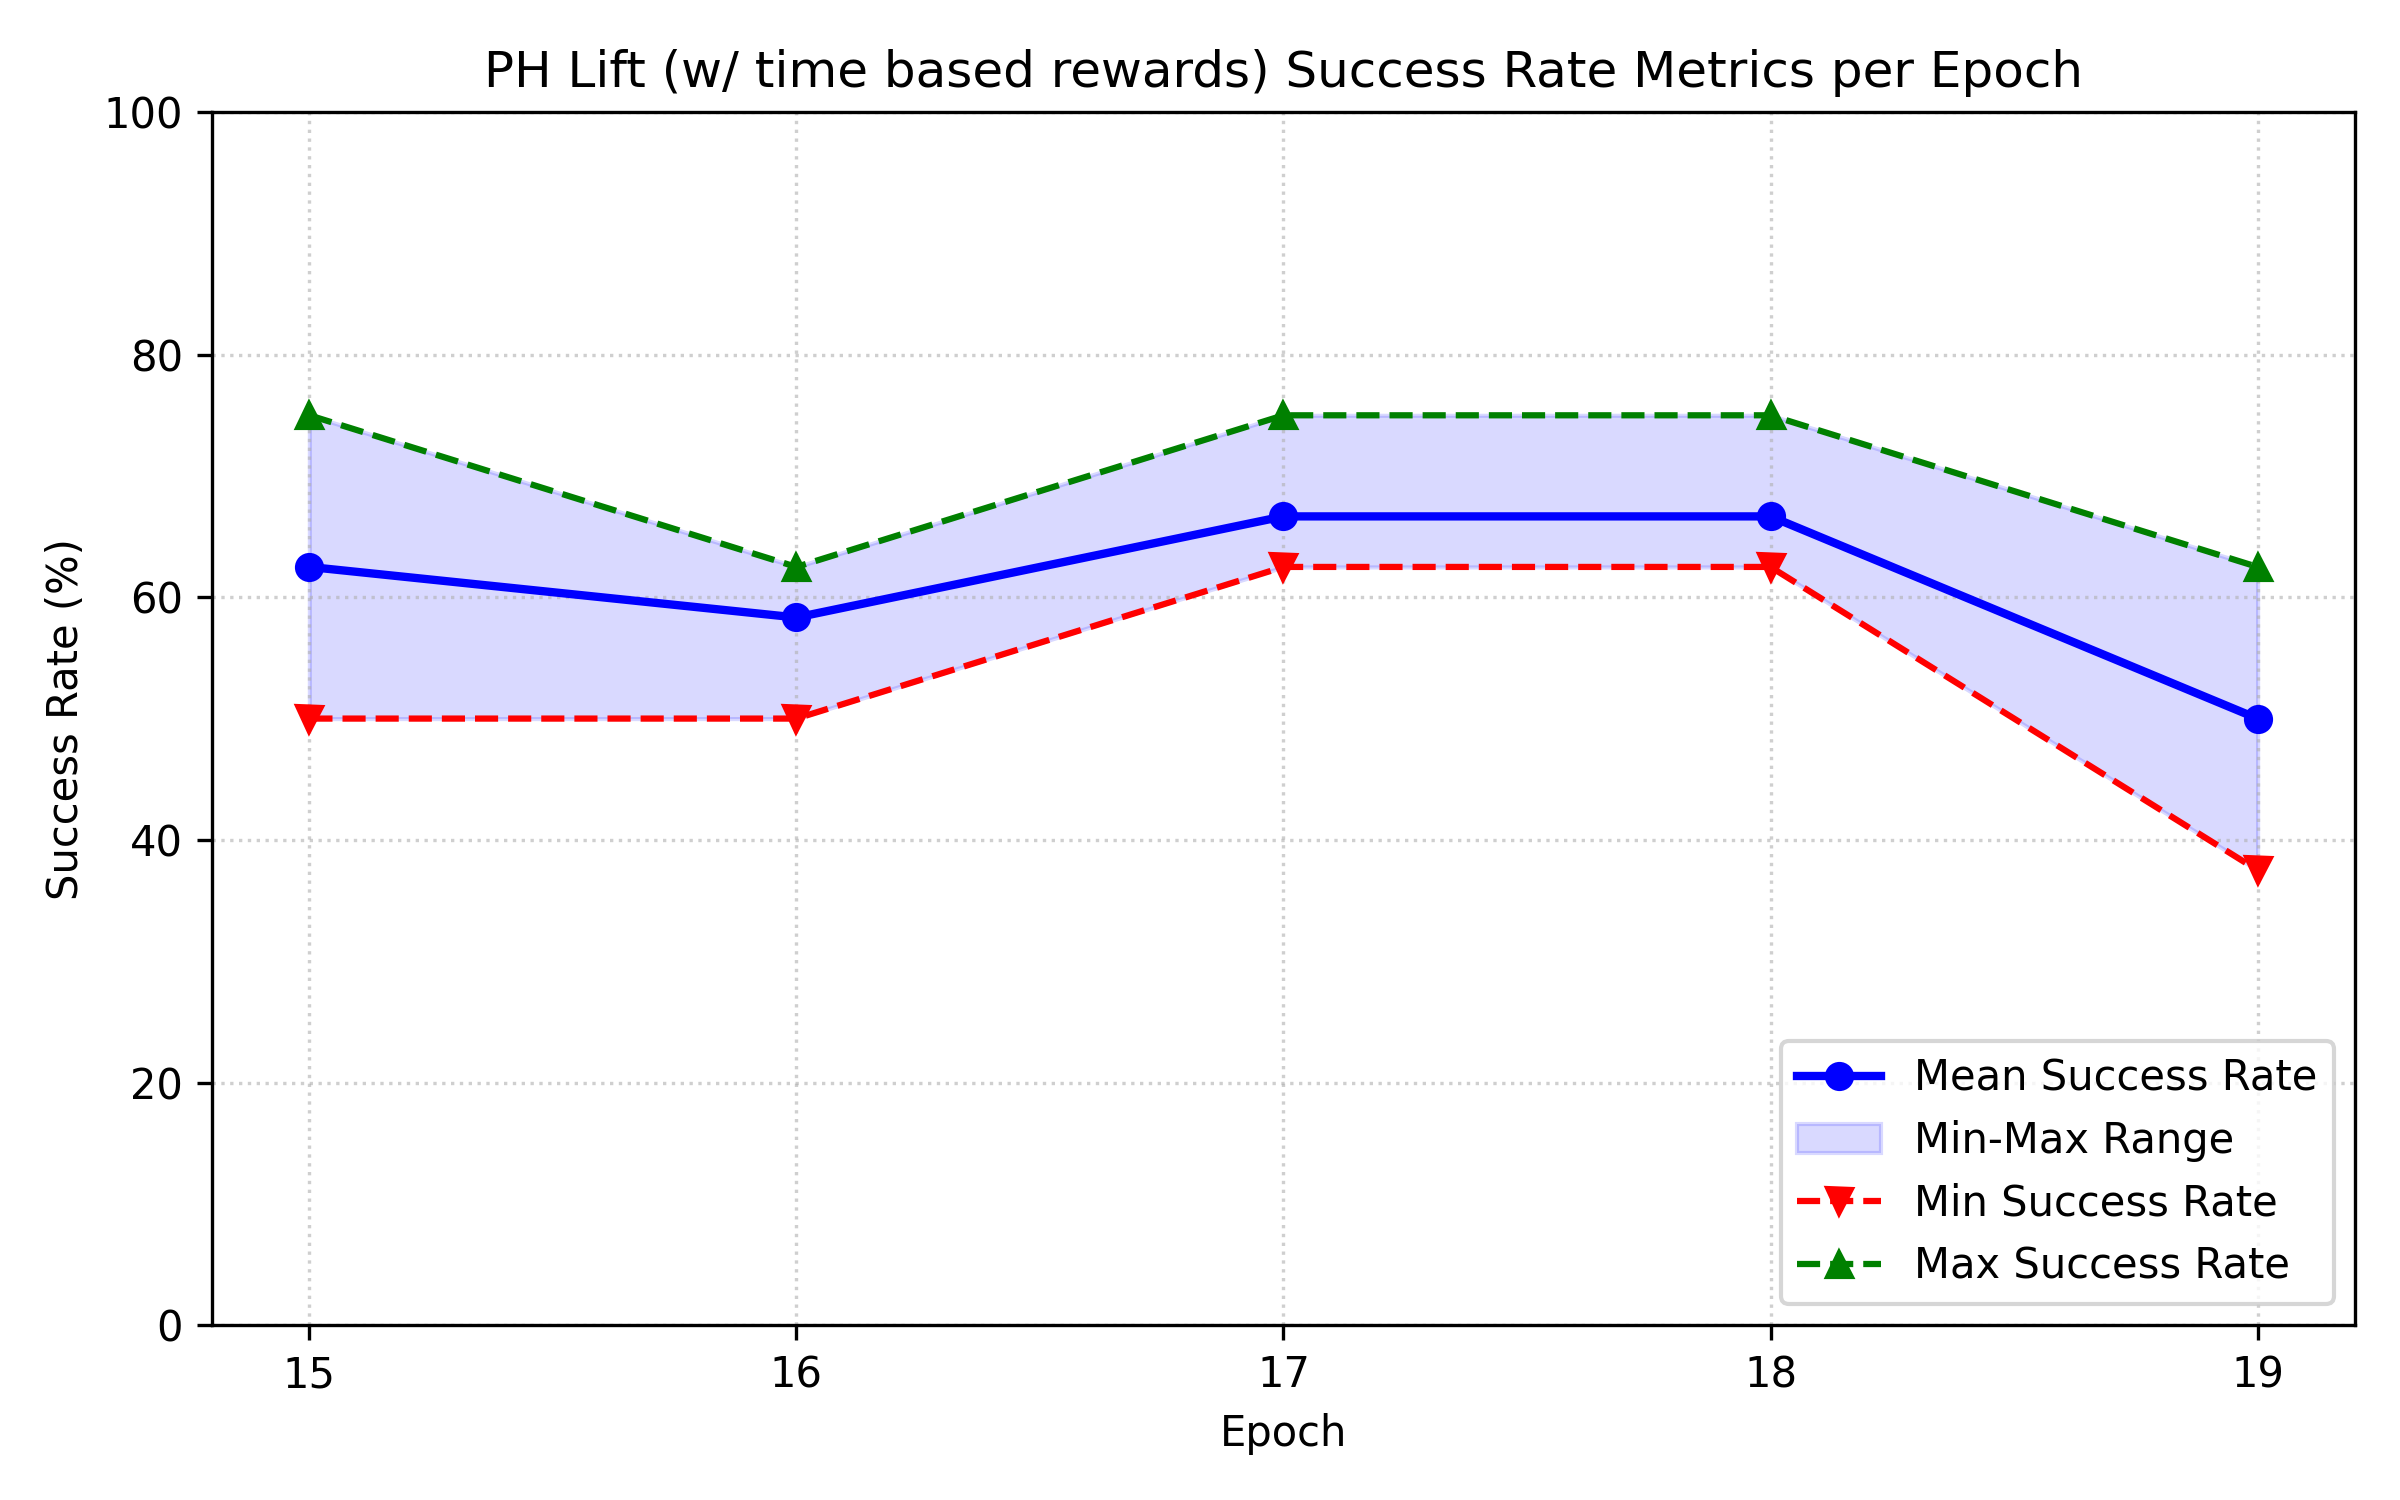
\includegraphics[width=\textwidth]{images/plots/time_based.png}
    \caption{Performance of the model trained with in-context prompts and time based rewards on the block lifting task (PH dataset).}
\end{figure}
\begin{figure}[htbp]
    \centering
    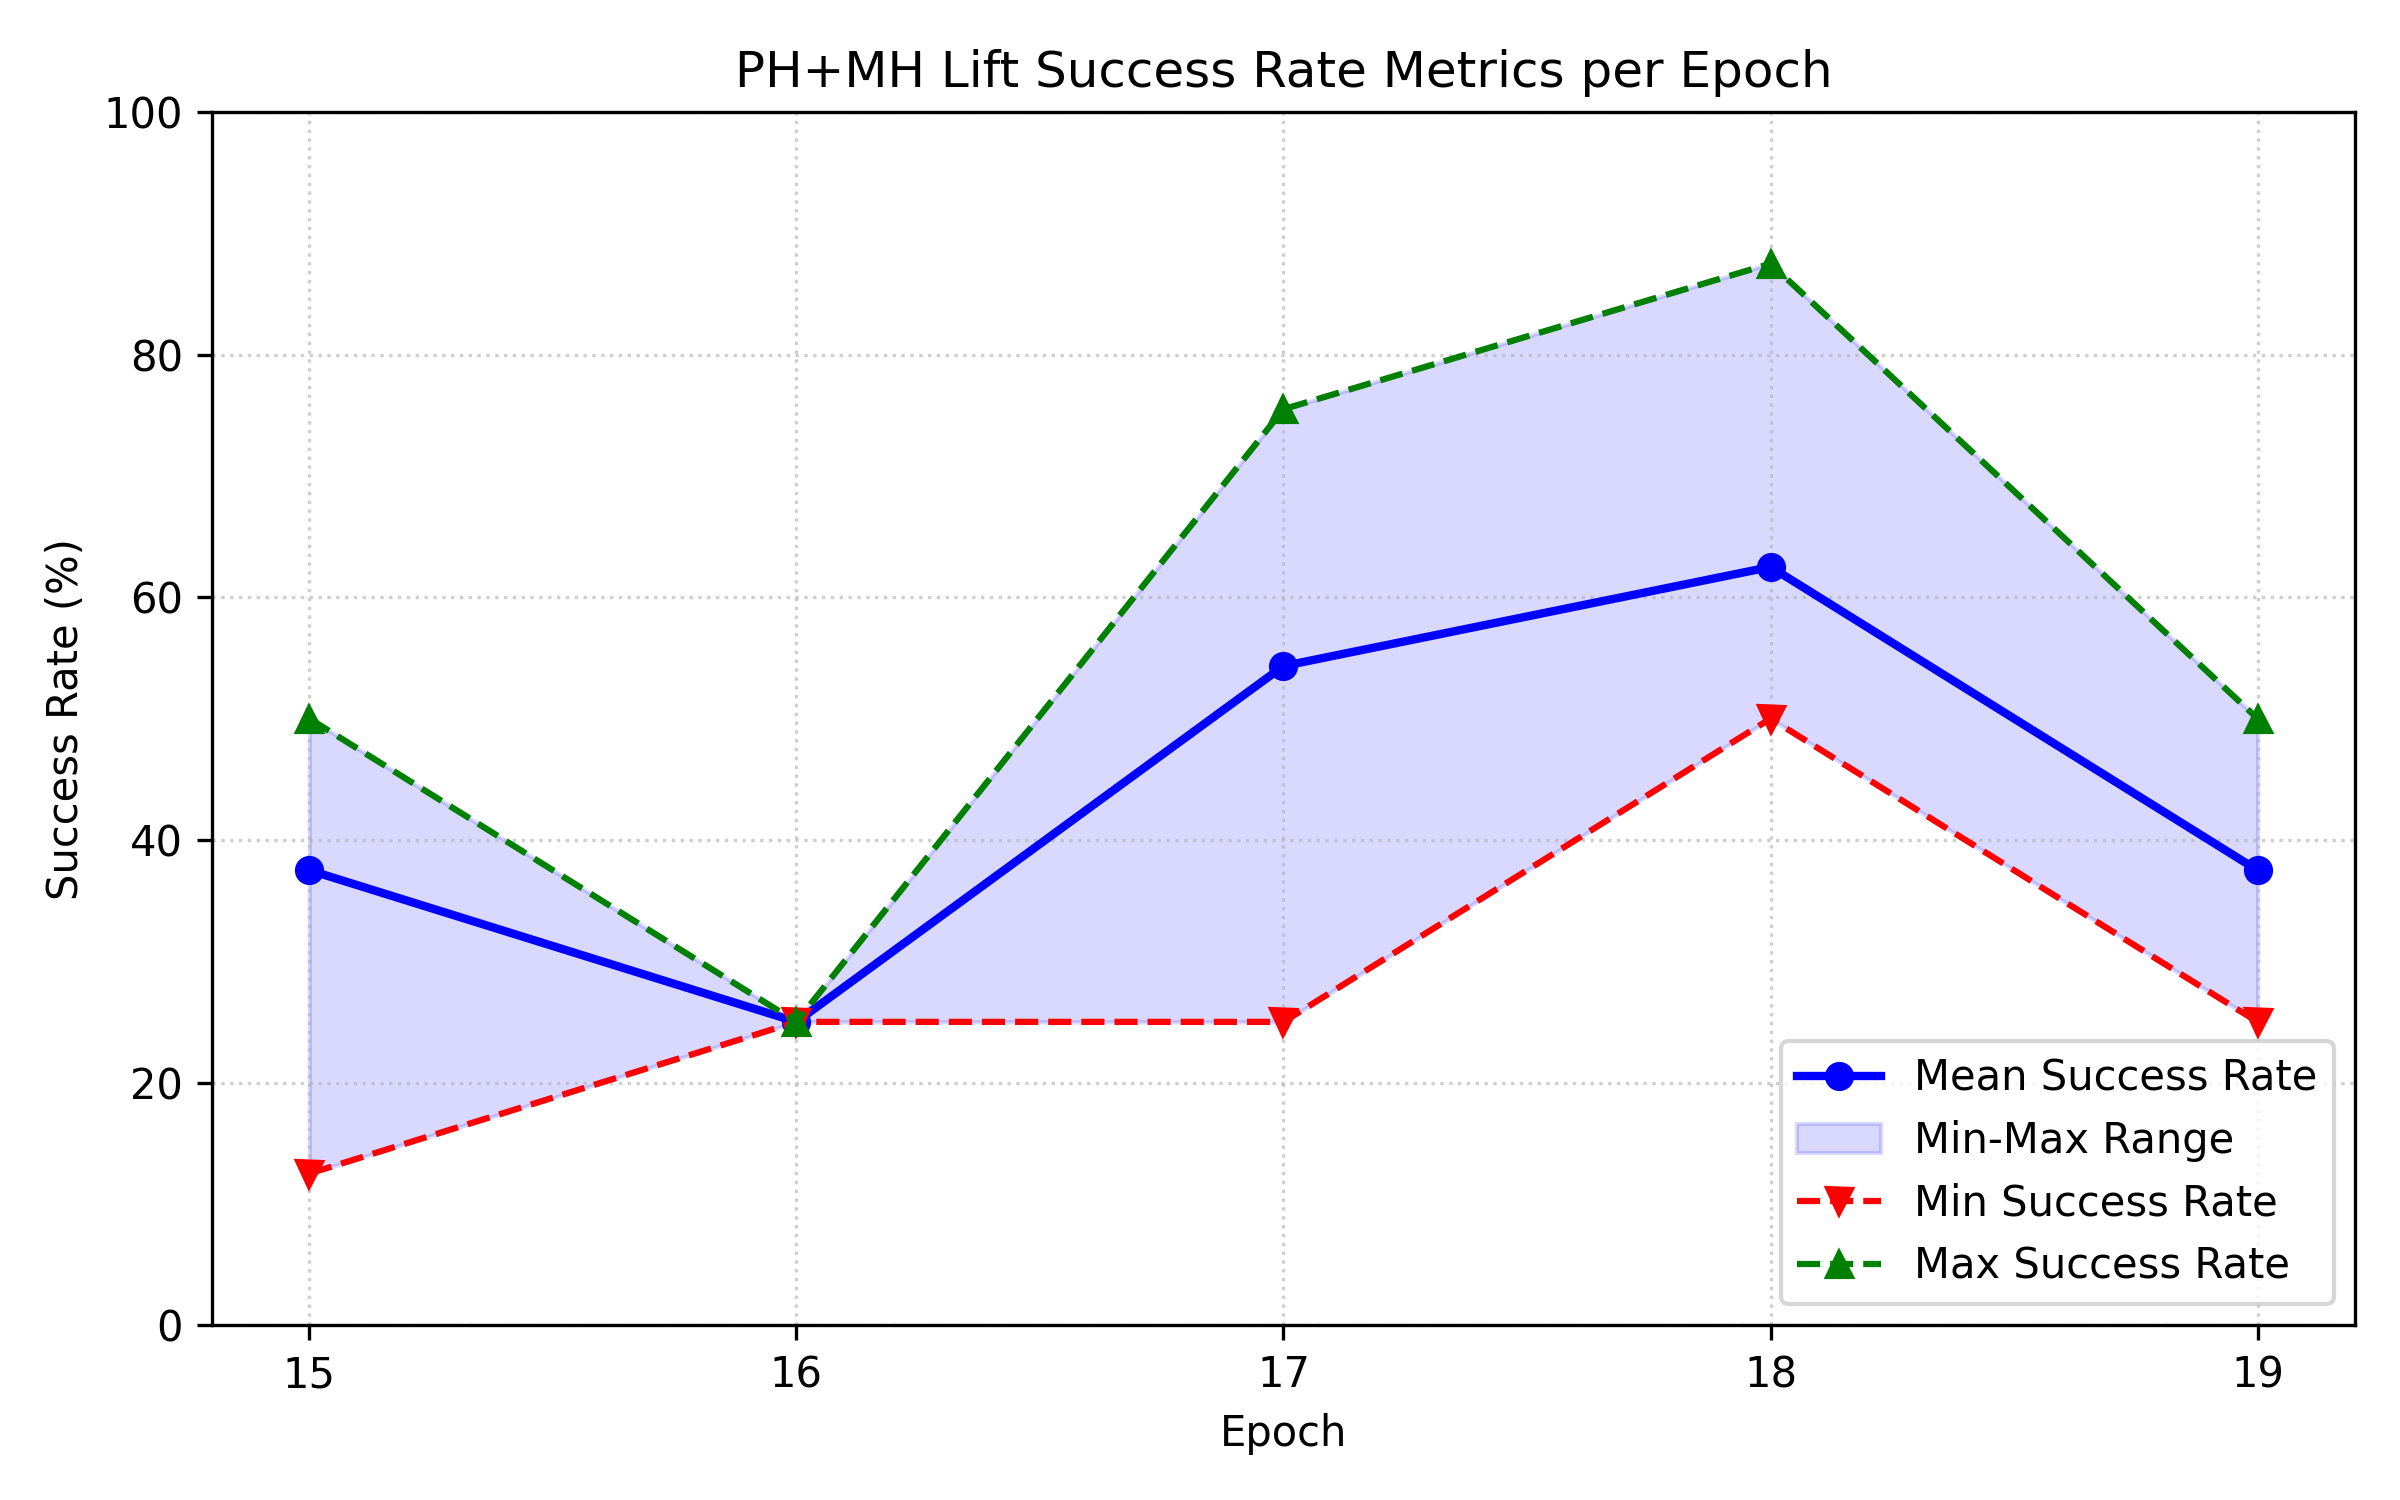
\includegraphics[width=\textwidth]{images/plots/icl_with_mh.png}
    \caption{Performance of the model trained with in-context prompts and time based rewards on the block lifting task (PH + MH dataset).}
\end{figure}

\begin{figure}[htbp]
    \centering
    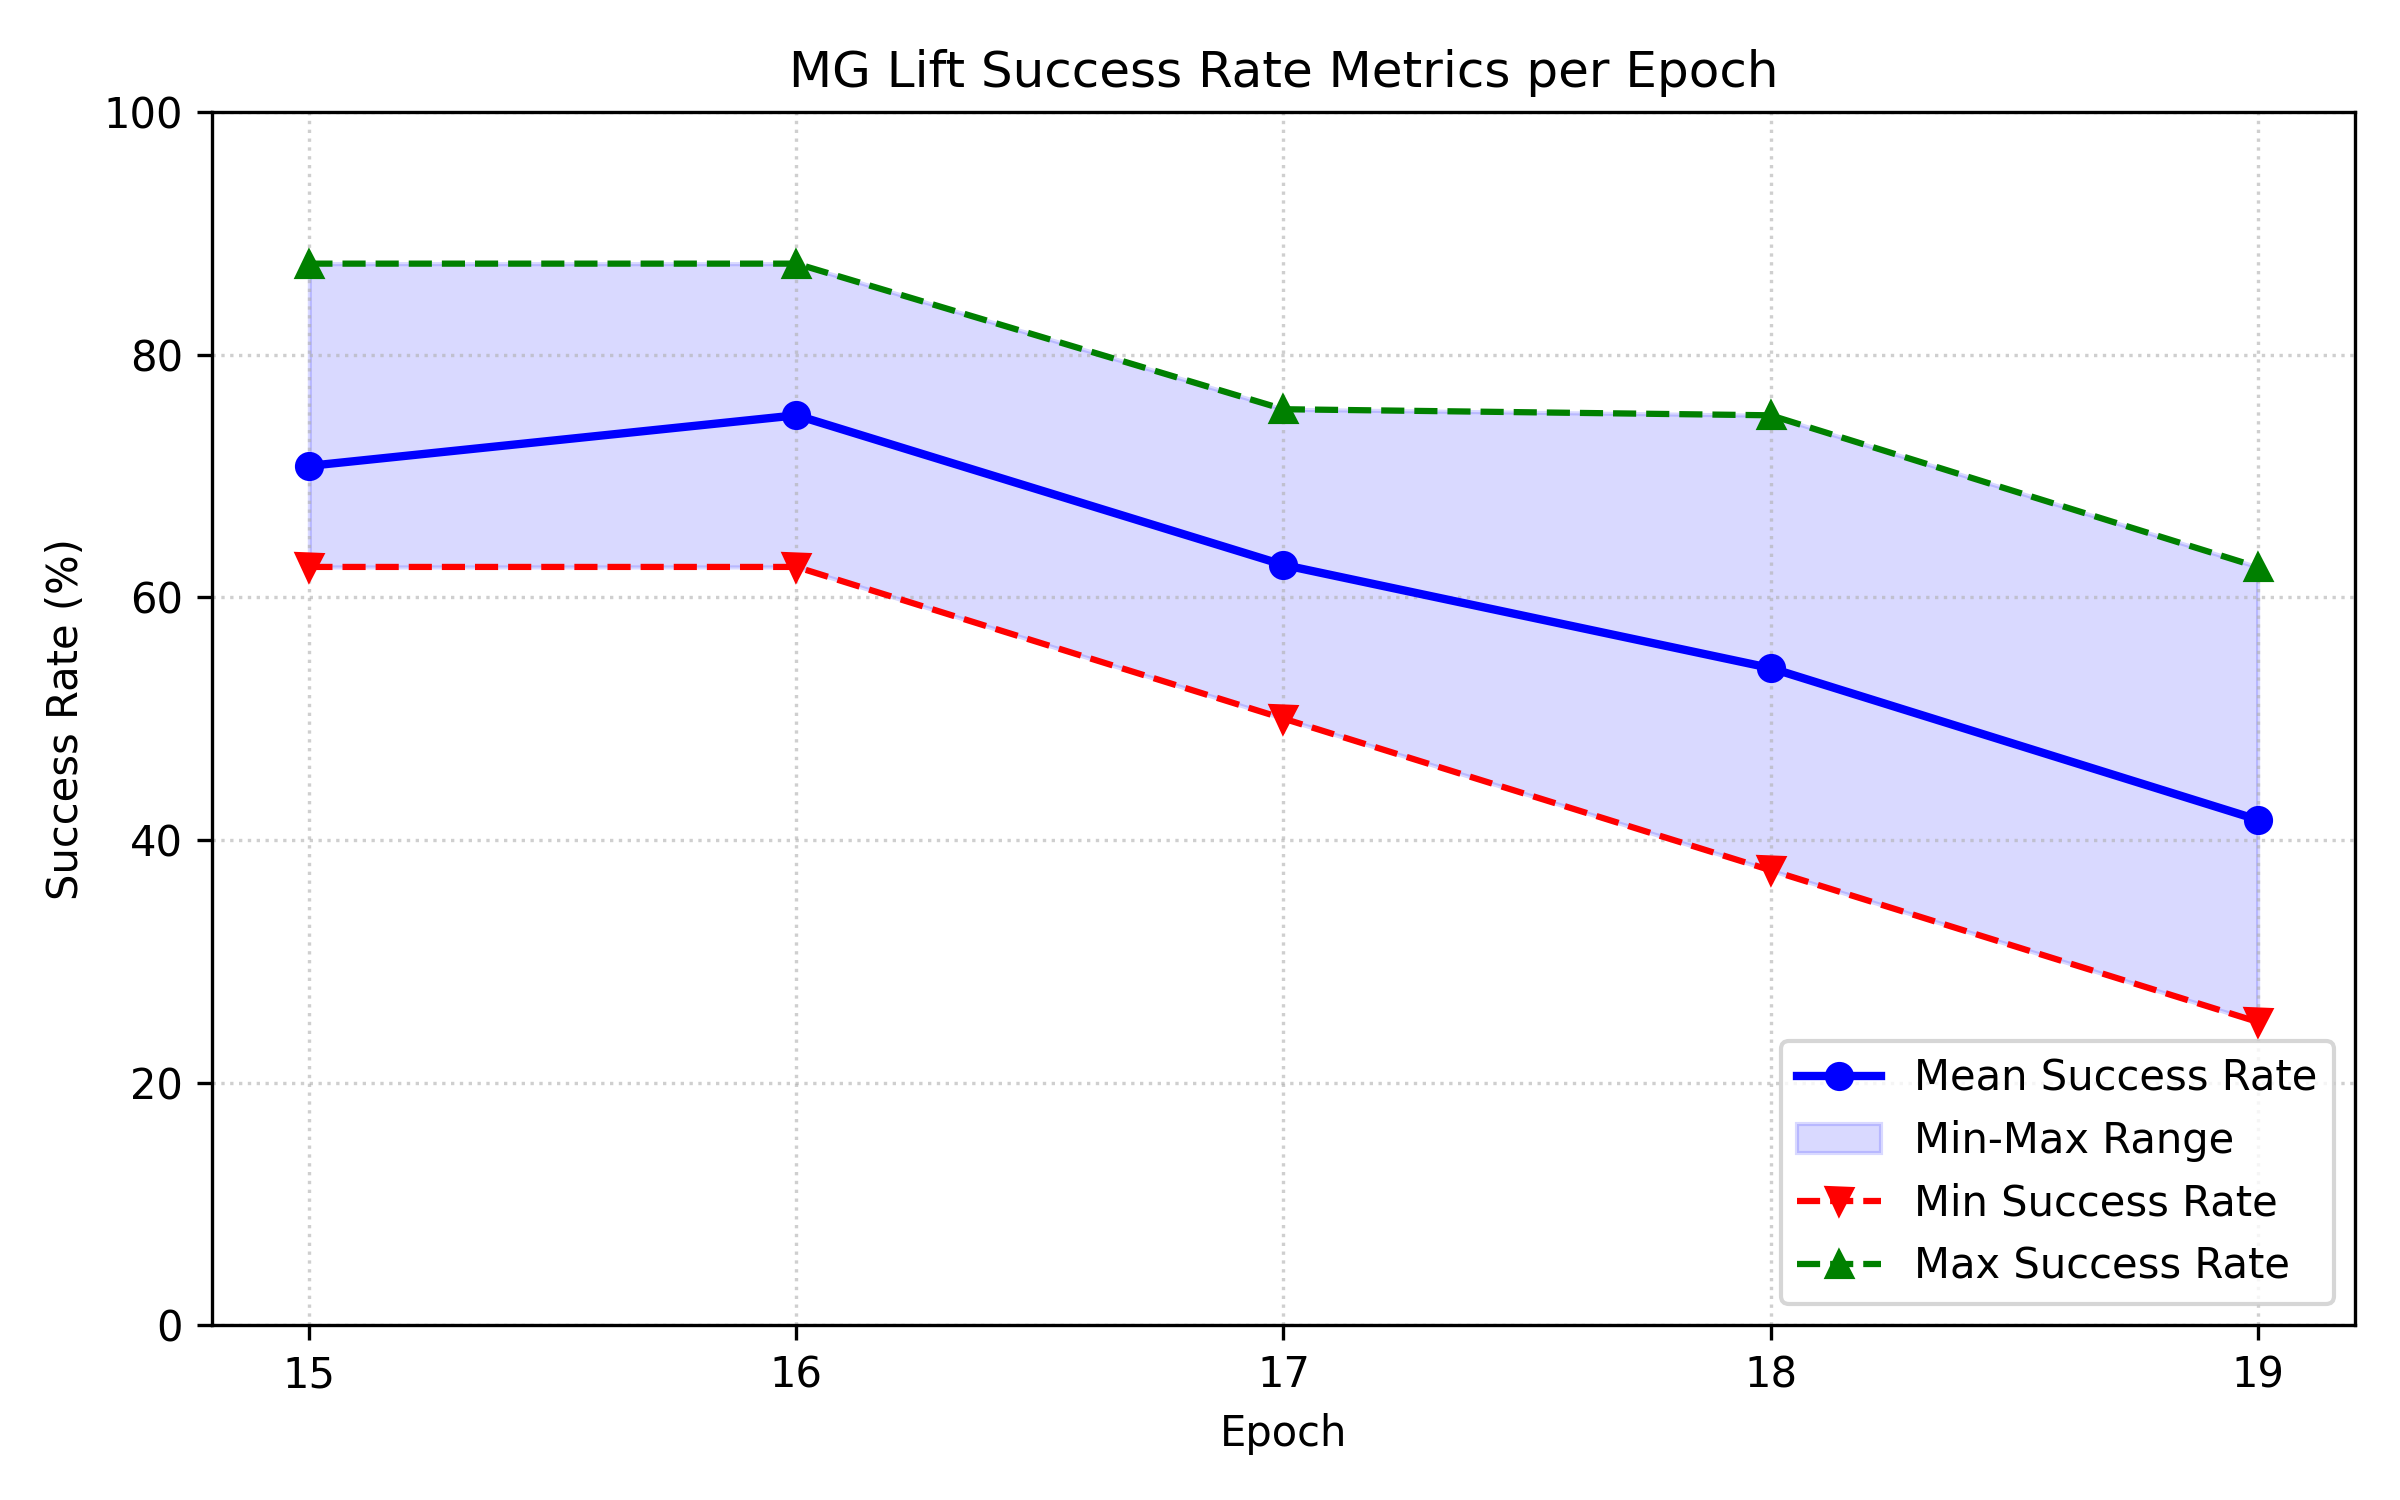
\includegraphics[width=\textwidth]{images/plots/icl_with_mg.png}
    \caption{Performance of the model trained with in-context prompts and time based rewards on the block lifting task (MG dataset).}
\end{figure}

\subsection{In-Context Learning}
All previously described models trained with in-context prompts, were evaluated on the block stacking task and achieved $\sim$ 0\% success rate.
They were prompted with a block stacking trajectory, but were unable to produce a successful one.

Instead of relying on pure in-context learning we tried adding a small sample of the block stacking demonstrations to the training data.
Their representation in the dataset was small (10 block stacking vs 200 block lifting), however we attempted to balance it with weighted sampling.
This resulted in improved performance on the main lifting task, and a glimpse of generalization with nonzero, $\sim$ 10\%, stacking success rate (see Figure 12).

We see it as an interesting achievement, because the 10 demonstrations alone weren't enough to train a working model, but mixing them into demonstrations of a much easier task sufficed.
This might suggest that there exists a possibility for bootstrapping - 10 manually collected demonstrations of a new task are enough for the model to incrementally produce its new training data. 

\begin{figure}[htbp]
    \centering
    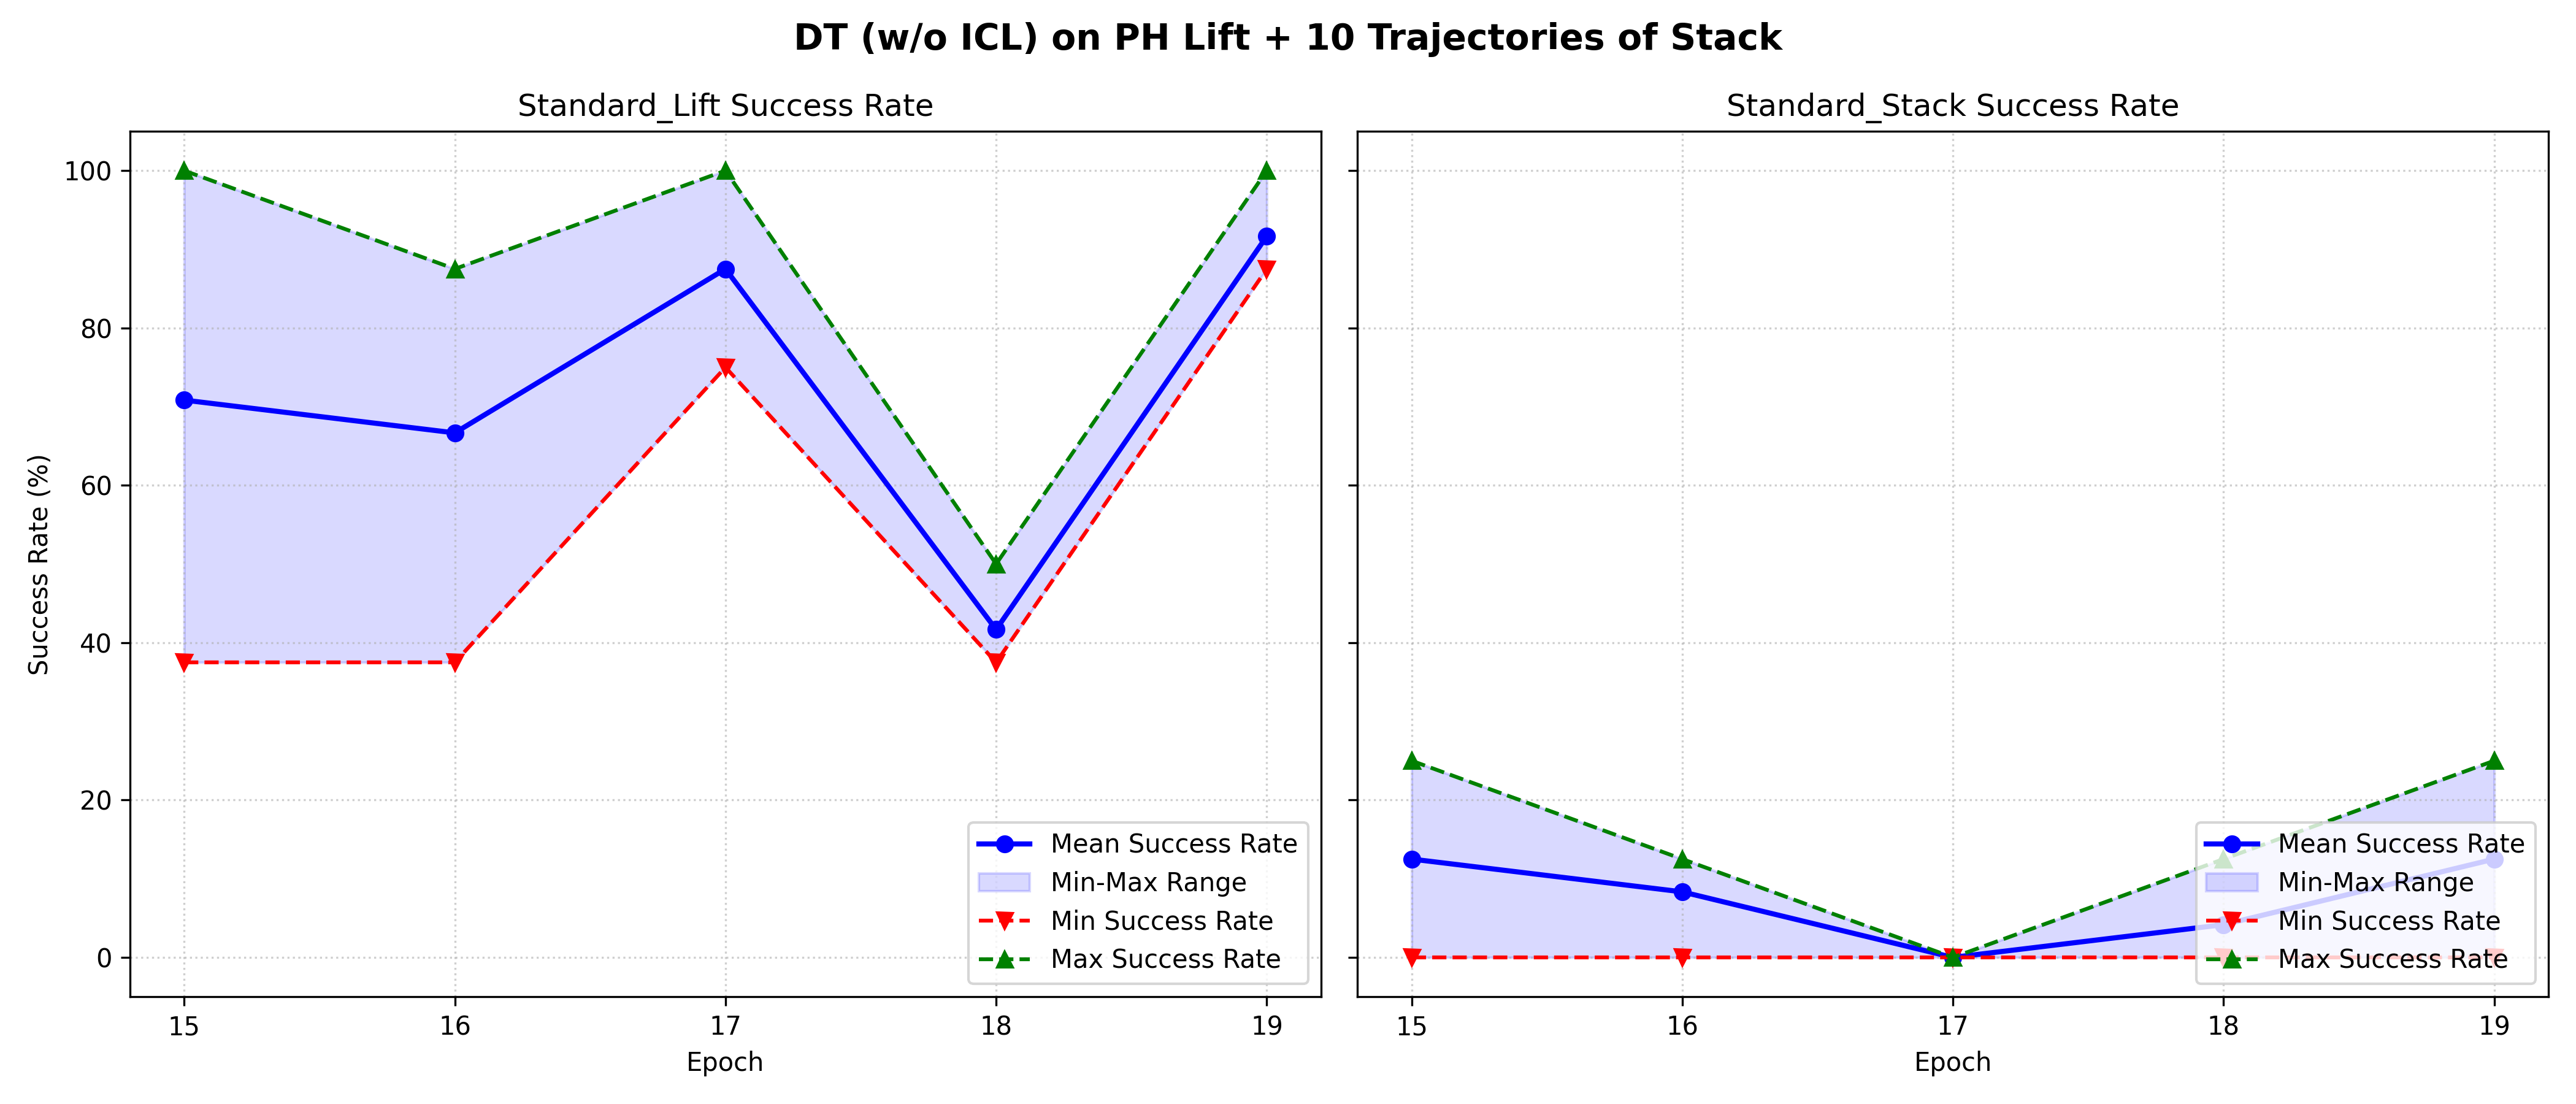
\includegraphics[width=\textwidth]{images/plots/lift_and_stack.png}
    \caption{Performance of the model trained on the block lifting (PH) and block stacking tasks.}
\end{figure}

\section{In Context Learning - Cross-embodiment Generalization}
TODO

\section{Conclusions}


\end{document}
